% RLJ main.tex Version 2026.1

\documentclass[10pt]{article} % For LaTeX2e

%%%%%%%%%%%%%%%%%%%%%%%%%%%%%%%%%%%%%%%%%%%%%%%%%%%%%%%%%%%%%%%%
% AUTHOR: Select ONE option:
%      [accepted]{rlj} --> for camera ready (after peer review, if accepted)
%      {rlj}           --> for submission
%      [preprint]{rlj} --> to de-anonymize and remove references to RLJ/RLC
%%%%%%%%%%%%%%%%%%%%%%%%%%%%%%%%%%%%%%%%%%%%%%%%%%%%%%%%%%%%%%%%
% \usepackage{rlj}           % Should be uncommented for submission
%\usepackage[accepted]{rlj} % Should be uncommented for the camera-ready
\usepackage[preprint]{rlj} % Should be uncommented for preprint versions


%%% Nuria added: Force the header (running title) back on for preprint mode
% 
\makeatletter
\if@preprint
    \lhead{\therunningtitle} % Puts title in the left
\fi
\makeatother



%%%%%%%%%%%%%%%%%%%%%%%%%%%%%%%%%%%%%%%%%%%%%%%%%%%%%%%%%%%%%%%%
% WARNING: The following packages are already included in the
%          rlj.sty style file:
%
%  1. fancyhdr  - For controlling header/footers
%  2. natbib    - For formatting the bibliography
%  3. enumitem  - To customize the appearance of lists
%  4. fontenc (with option [T1]) - Allows for proper hyphenation and accents
%  5. times     - Times new roman font
%  6. ragged2e  - Used to justify text
%  7. tcolorbox - Used to create boxes on cover page
%  8. hyperref  - Configures hyperlinks throughout (e.g., links to references)
%  9. xcolor    - Used to define custom colors for links and boxes
%  10. amsmath  - Not used, but conflicts with lineno, so we include (and patch) it for authors
%  11. etoolbox - Included in the amsmath + lineno patch
%  12. lineno   - For adding line numbers when in submission
%
% You do not need to include them again in your main.tex.
% Including them again may lead to conflicts or compilation errors.
% Additionally, avoid loading packages that might conflict with these.
%%%%%%%%%%%%%%%%%%%%%%%%%%%%%%%%%%%%%%%%%%%%%%%%%%%%%%%%%%%%%%%%

%%%%%%%%%%%%%%%%%%%%%%%%%%%%%%%%%%%%%%%%%%%%%%%%%%%%%%%%%%%%%%%%
% Recommended (but not required) packages
%%%%%%%%%%%%%%%%%%%%%%%%%%%%%%%%%%%%%%%%%%%%%%%%%%%%%%%%%%%%%%%%
\usepackage{amssymb}            % Defines common symbols like \mathbb R
\usepackage{mathtools}          % Extends amsmath, providing common math tools
\usepackage{mathrsfs}           % Enables \mathscr, which can work in cases that \mathcal does not
%\mathtoolsset{showonlyrefs}     % Only number equations that are referenced (optional)
\usepackage{graphicx}           % For including images
\usepackage{subcaption}         % Allows for the use of subfigures and subcaptions
\usepackage[space]{grffile}     % For spaces in image names
\usepackage{url}                % For displaying URLs
\usepackage{lipsum}             % For placeholder text

%%%%% USER ADDED
\usepackage{float}
\usepackage{multirow}
\usepackage{tabularx}
\usepackage{threeparttable}
\usepackage{booktabs}


%%% Nuria
\usepackage{xspace}
\setlength{\marginparwidth}{2cm}
\usepackage[textsize=tiny]{todonotes}
% \usepackage[textsize=small, disable]{todonotes}
\usepackage{hyperref} % Optional, but usually used together
\usepackage{cleveref}
\newcommand{\algo}[1]{\textsc{#1}}
% \newcommand{\method}{\algo{FANCYNAME}\xspace}
% \newcommand{\method}{\algo{FANCYNAME}}
\newcommand{\method}{\mbox{\algo{FB-MEBE}}\xspace}

% Graph
\def\gA{{\mathcal{A}}}
\def\gB{{\mathcal{B}}}
\def\gC{{\mathcal{C}}}
\def\gD{{\mathcal{D}}}
\def\gE{{\mathcal{E}}}
\def\gF{{\mathcal{F}}}
\def\gG{{\mathcal{G}}}
\def\gH{{\mathcal{H}}}
\def\gI{{\mathcal{I}}}
\def\gJ{{\mathcal{J}}}
\def\gK{{\mathcal{K}}}
\def\gL{{\mathcal{L}}}
\def\gM{{\mathcal{M}}}
\def\gN{{\mathcal{N}}}
\def\gO{{\mathcal{O}}}
\def\gP{{\mathcal{P}}}
\def\gQ{{\mathcal{Q}}}
\def\gR{{\mathcal{R}}}
\def\gS{{\mathcal{S}}}
\def\gT{{\mathcal{T}}}
\def\gU{{\mathcal{U}}}
\def\gV{{\mathcal{V}}}
\def\gW{{\mathcal{W}}}
\def\gX{{\mathcal{X}}}
\def\gY{{\mathcal{Y}}}
\def\gZ{{\mathcal{Z}}}

% SET
\def\sR{{\mathbb{R}}}

% Argmin, argmax operators
\DeclareMathOperator*{\argmax}{arg\,max}
\DeclareMathOperator*{\argmin}{arg\,min}



% Legends:
\definecolor{ourblue}{rgb}{0.368,0.507,0.71}
\definecolor{ourorange}{rgb}{0.881,0.611,0.142}
\definecolor{ourgreen}{rgb}{0.56,0.692,0.195}
\definecolor{ourred}{rgb}{0.923,0.386,0.209}
\definecolor{ourdarkred}{rgb}{0.7373, 0.3765, 0.2549}
\usepackage{dashrule}
\newcommand{\nuria}[1]{\textcolor{red}{#1}}
\usepackage{algorithm, algorithmic}


%%%%%%%%%%%%%%%%%%%%%%%%%%%%%%%%%%%%%%%%%%%%%%%%%%%%%%%%%%%%%%%%
% AUTHOR: Fill in the following meta-data
%%%%%%%%%%%%%%%%%%%%%%%%%%%%%%%%%%%%%%%%%%%%%%%%%%%%%%%%%%%%%%%%

% Enter the title of your paper:
\title{Maximum Entropy Behavior Exploration for \\ Sim2Real Zero-Shot Reinforcement Learning} %Just an idea

% The "running title" will be displayed in the header on every-other page.
% It is typically either the same as the title or a shorter version of the title.
% Enter your running title here:
\setrunningtitle{Maximum Entropy Behavior Exploration for Sim2Real Zero-Shot Reinforcement Learning}

% WARNING: Authors must not appear in the submitted version. They should be hidden
% as long as the rlj package is used without the [accepted] or [preprint] options.
% Non-anonymous submissions will be rejected without review.

% Enter the author names below. 
% NOTE: Denote affiliations using superscripts as in the provided example.
% NOTE: Use \textscript{1,2,3} instead of $^{1,2,3}$.
%       - Failure to do so will cause affiliation superscripts to appear on the cover page for camera-ready and preprint versions.
\author{Jiajun Hu\textsuperscript{1,$\dagger$}, Núria Armengol Urpí\textsuperscript{2,3,$\dagger$}, Jin Cheng\textsuperscript{2}, Stelian Coros\textsuperscript{2}}

% NOTE: For camera-ready and preprint versions, the cover page includes author names but not affiliations.
% It automatically removes the superscripts for affiliations.
% If the automatic process breaks (e.g., if an author name should include a superscript), you can manually define the author string to appear on the cover page by uncommenting the following line.
%\coverPageAuthor{Marlos C. Machado, Philip S. Thomas, Lorem Ipsum}

% Author emails, which can be clustered if they have shared endings as in this example
\emails{jiajun.hu@epfl.ch, \ \{nuriaa,jcheng\}@ethz.ch}

% Author affiliations, in the order the occur
% The inclusion of state/province, etc. is optional.
% The inclusion of multiple affiliations is optional.
%   - List multiple affiliations with comma-separated numbers as in the example.
\affiliations{
$^{1}$\textbf{EPFL}\\
$^{2}$\textbf{ETH Zurich}\\
$^{3}$\textbf{Max Planck Institute for Intelligent Systems}\\
% The following two lines are optional and can be commented out
% \par % If including additional comments like below, use \par to add some whitespace. 
$^\dagger$Corresponding authors
}

\contribution{
We identify ineffective exploration as a primary bottleneck when deploying online Forward-Backward (FB) representations on real quadrupedal robots, characterized by poor state coverage and degenerate locomotion behaviors.
}
{
Prior work \citep{touati2023does} has demonstrated the effectiveness of FB in simulated control benchmarks, but its exploration properties in real-world robotic systems have not been systematically examined.
}

\contribution{
% We introduce a Normalizing Flow (NF)--based mechanism to model and reshape the latent variable $z$ distribution in FB, 
We introduce an entropy maximization sampling strategy for online exploration, improving exploration without relying on external motion capture priors.
}
{
Existing real-robot FB \citep{li-2025} approaches depend on motion capture datasets, which limit applicability when such priors are unavailable.
}

\contribution{
% We demonstrate one of the first deployments of online FB on a real quadrupedal robot without motion capture data, showing that structured latent exploration enables stable training and improved locomotion performance on hardware.
To the best of our knowledge, we demonstrate the first deployment of online FB on a real quadrupedal robot without external dataset or motion capture data.
}
{
% Previous deployments of FB-based methods on physical robots have relied on large-scale motion capture datasets to facilitate exploration.
Previous deployments of zero-shot reinforcement learning methods on physical robot have taken place on humanoid robots, for which the availability of large-scale motion capture datasets facilitate exploration.
}

% Include a list of keywords for the topic of the paper:
\keywords{unsupervised RL, exploration, zero-shot, quadruped, sim2real} % Your keywords

% Define the summary that appears on the cover page.
\summary{Zero-shot reinforcement learning aims to learn policies that can adapt to arbitrary reward functions without retraining. Forward-Backward (FB) representations achieve this by learning successor measures, enabling efficient reward inference at test time. However, in the absence of external datasets, we observe that undirected exploration in FB often suffers from ineffective exploration, leading to distributional shrinkage and poor coverage of dynamically diverse states. In this work, we investigate the exploration bottleneck of \textit{online} FB training for quadrupedal control. We show that the empirical training data distribution progressively collapses toward low-diversity regions, significantly degrading zero-shot performance. To address this, we propose \method, a method for unsupervised behavior exploration,  that promotes exploration towards maximizing the entropy of the achieved behavior distribution. Our method actively expands state coverage without altering the FB objective. Empirical results demonstrate improved data diversity, enhanced zero-shot performance, and stable locomotion behaviors in simulated downstream tasks, and seamless transfer of recovered policies to hardware.  
}

%%%%%%%%%%%%%%%%%%%%%%%%%%%%%%%%%%%%%%%%%%%%%%%%%%%%%%%%%%%%%%%%
%% Begin document, create title and abstract
%%%%%%%%%%%%%%%%%%%%%%%%%%%%%%%%%%%%%%%%%%%%%%%%%%%%%%%%%%%%%%%%
\begin{document}

% \makeCover  % Create the cover page
\maketitle  % Make the title section

\begin{abstract}
Zero-shot reinforcement learning (RL) algorithms aim to learn a family of policies from a reward-free dataset, and recover optimal policies for any reward function directly at test time. Naturally, the quality of the pretraining dataset determines the performance of the recovered policies across tasks. However, pre-collecting a relevant, diverse dataset without prior knowledge of the downstream tasks of interest remains a challenge. 
In this work, we study \textit{online} zero-shot RL for quadrupedal control on real robotic systems, building upon the Forward-Backward (FB) algorithm. We observe that undirected exploration yields low-diversity data, leading to poor downstream performance and rendering policies impractical for direct hardware deployment. Therefore, we introduce ~\method, an online zero-shot RL algorithm that combines an unsupervised behavior exploration strategy with a regularization critic. \method promotes exploration by maximizing the entropy of the achieved behavior distribution. Additionally, a regularization critic shapes the recovered policies toward more natural and physically plausible behaviors. 
We empirically demonstrate that \method achieves and improved performance compared to other exploration strategies in a range of simulated downstream tasks, and that it renders natural policies that can be seamlessly deployed to hardware without further finetuning. Videos and code available on our \href{https://math-286-pro.github.io/FB-MEBE-Web/}{website}.

\begin{figure}[H]
    \centering
    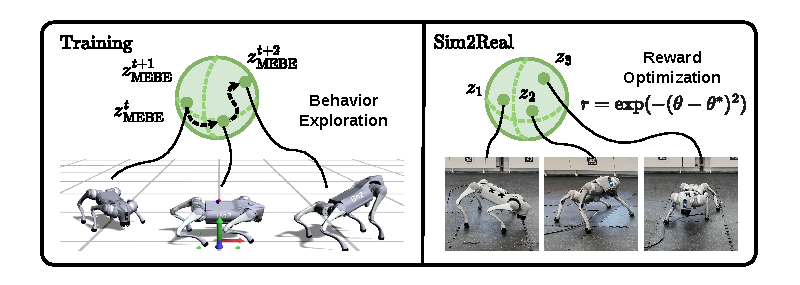
\includegraphics[width=1.0\linewidth]{figure/FB-Teaser.pdf} 
    \caption{\method improves behavior exploration by maximizing the behavior entropy during training. With the regularizer critic, \method achieves zero-shot hardware deployment by optimizing reward at inference time.}
    \label{fig:teaser}
\end{figure}
\end{abstract}



%%%%%%%%%%%%%%%%%%%%%%%%%%%%%%%%%%%%%%%%%%%%%%%%%%%%%%%%%%%%%%%%
%% Section: Introduction (Test)
%%%%%%%%%%%%%%%%%%%%%%%%%%%%%%%%%%%%%%%%%%%%%%%%%%%%%%%%%%%%%%%%
\section{Introduction}
Zero-shot reinforcement learning (RL) \citep{touati2023does} has emerged as a promising paradigm for developing general-purpose agents. 
By learning successor measures that decouple dynamics from rewards, these methods generate near-optimal policies for a big family of reward functions at test time, with minimal amount of computation and relying solely on unlabeled, precollected data. 
This departs from standard, fixed-reward-based RL \citep{sutton1998introduction}, which typically requires training a new policy whenever the objective changes. 
As these methods scale beyond complex and broader settings, they are usually referred to as Behavior Foundation Models (BFMs) \citep{tirinzoni2025zeroshot}. Such generalization capabilities are particularly appealing for robotics, where usually learning relevant policies involves tedious reward engineering. While general-purpose foundation models trained on vast amounts of (un)labeled data have emerged as a promising paradigm for robotic manipulation \citep{intelligence2025pi, brohan2023rt,kim2024openvla}, the application of BFMs for legged systems still remains underexplored.
One of the main bottlenecks is the reliance on large, diverse, task-agnostic precollected datasets \citep{laskin2021urlb}, which are often unavailable at scale for legged robots. 

Recently, \citet{tirinzoni2025zeroshot} proposed an online zero-shot RL algorithm grounding policy learning and exploration towards an external motion capture dataset. Based on this idea, BFM-Zero \citep{li-2025} represents an early effort to transfer such zero-shot RL methods to a humanoid robot. However, these methods still rely on supervision from external datasets. 
In this paper, we focus on the quadrupedal setting. We observe that naive deployment of online FB suffers from ineffective exploration and has difficulties in discovering the sparse manifold of stable locomotion. In contrast to previously explored efforts \citep{li-2025}, large motion capture dataset are not readily available for quadrupedal robots and thus cannot be used to regularize exploration.

We thus propose \method (Maximum Entropy Behavior Exploration), an online zero-shot RL framework based on the forward-backward (FB) algorithm \citep{touati2021learning}, which does not require access to external datasets.


\method leverages an unsupervised behavior exploration strategy that guides the agent to maximize the entropy of the achieved behavior distribution,  similarly to \citep{pitis2020maximum}. 
Closest to our work, \citep{urpiepistemically} framed the exploration problem in FB as a minimization of the epistemic uncertainty that the algorithm has of its representations.
In our case, we adopt a frequentist approach, guiding the agent towards reaching behaviors with low visitation count. This strategy implicitly induces a curriculum on the behaviors with which to explore next, effectively pushing the frontier of achievable behaviors. Furthermore, to ensure that the manifold of solutions induced by the unsupervised strategy is aligned with the downstream task of interest,  we embed an inductive bias to favor physically plausible behaviors via a behavior regularizer. This forces the recovered policies to maintain their zero-shot capabilities while being readily deployable to real hardware. 

We empirically demonstrate that \method achieves improved downstream performance compared to other exploration strategies in simulation in a range of downstream tasks, and that it renders policies with natural behaviors that can be seamlessly deployed to hardware without further finetuning.
To the best of our knowledge, this is the second instantiation of the FB algorithm on real robotic systems, and the very first to do so entirely online without relying on prior external datasets.
In summary, in this work we provide a maximum entropy exploration strategy for efficiently learning FB representations online that %\begin{enumerate}[label=\alph*)]
a) exhibits improved downstream performance in quadruped tasks in simulation compared to other exploration alternatives,
b) renders policies with smooth, physically plausible behaviors and 
c) enables the direct, zero-shot deployment of recovered policies onto real hardware.



%%%%%%%%%%%%%%%%%%%%%%%%%%%%%%%%%%%%%%%%%%%%%%%%%%%%%%%%%%%%%%%%
%% Section: Related Work (Test)
%%%%%%%%%%%%%%%%%%%%%%%%%%%%%%%%%%%%%%%%%%%%%%%%%%%%%%%%%%%%%%%%
\section{Related Work}
\paragraph{Zero-shot RL} Zero-shot RL spans a range of methods that train agents on unsupervised data to enable zero-shot generalization to a wide range of tasks. It traces back to successor representations \citep{dayan1993improving}, a direct extension to the continuous MDPs being the successor features \citep{barreto2017successor}. In \citep{borsauniversal}, given a handcrafted feature map on the states, it defines the set of all reward functions that lie on the linear span of the features. Several extensions have been proposed to learn the features map \citep{hansen2019fast, laskin2021urlb}. The forward backward algorithm, FB \citep{touati2021learning, touati2023does}, applies a similar idea to a finite-rank model of successor measures, adopting a contrastive loss computing pairwise dot-products across each training batch, and learns the feature map and corresponding successor features \textit{jointly}. FB has been subsequently extended to alternative parameterizations \citep{bagatella2025td, cetin25}, for zero-shot imitation \citep{pirotta2024fast}, offline training from low quality data \citep{jeen2023zero}, online training regularized with unlabeled expert data\citep{tirinzoni2025zeroshot}, training on environments with different dynamics \citep{bobrin2025zero}, extending it to optimising general utilities beyond linear RL \citep{bagatella2026soft}  online finetuning \citep{sikchi_fast_2025}, test-time task inference \citep{rupf2025optimistic}  or self-supervised exploration \citep{urpiepistemically, fb-dual-value}.
Other zero-shot methods are HILP \citep{park2024foundation}, that learn state features with a goal reaching loss in a latent space and PSM \citep{agarwal2024proto} learning an affine decomposition of the succesor measure for a discrete codebook of policies.

\paragraph{Exploration in unsupervised RL}
There has been vast work on exploration in unsupervised RL \citep{diayn, rnd, emergentoffdads, park_metra_2024} or unsupervised goal-conditioned RL focused on discovering a wide range of goals and learning corresponding goal-reaching policies \citep{mendonca2021discovering,bagaria2019option}, exploring with goals that have lower density \citep{pitis2020maximum, Skew-Fit, diaz2025discover, florensa2018automatic}.Most of these work, in contrast to zero-shot RL require separate methods for learning policies. Closest to our work, \citet{urpiepistemically} framed the exploration problem in online FB as a minimization of the epistemic uncertainty exploring with task embeddings that lead to the highest information gain and \citet{fb-dual-value} leverage RND for promoting data diversity.


%%%%%%%%%%%%%%%%%%%%%%%%%%%%%%%%%%%%%%%%%%%%%%%%%%%%%%%%%%%%%%%%
%% Section: Background (Test)
%%%%%%%%%%%%%%%%%%%%%%%%%%%%%%%%%%%%%%%%%%%%%%%%%%%%%%%%%%%%%%%%
\section{Background}

We consider a standard reward-free Markov decision process (MDP), defined by the tuple \mbox{$\gM = (\gS, \gA, P, \gamma, d_0)$}, where $\gS, \gA$ are the state and action space, $P$ is the transition kernel, $\gamma \in (0,1)$ is the discount factor and $d_0$ is the initial state distribution.
Given the MDP $\gM$, a policy \mbox{$\pi: \gS \rightarrow \Delta\gA$}, mapping states to probabilities over actions, its successor measure \citep{dayan1993improving, blier2021} for any initial state-action pair \mbox{$(s_0, a_0) \in \gS \times \gA$} is the discounted cumulative distribution of visiting future states when starting from state $s_0 \in \gS$, take action $a \in \gA$ and following policy $\pi$ thereafter. Formally, it is defined as
\begin{equation}
\label{eq:succesor_measure}
    M^\pi( X | s_0, a_0 ) = \sum_{t\geq0}\gamma^t P(s_{t+1} \in X | s_0, a_0, \pi) \quad \forall X \in \gS.
\end{equation}
Conveniently, the action-value function for policy $\pi$ and any reward function $r: \gS \rightarrow \sR$, can be expressed as
% The derivation of this equivalence is provided in Appendix~\ref{appendix:successor_q_derivation}.
\begin{equation}
\label{eq:q_from_successor}
Q_r^\pi(s,a) := \mathbb{E} \big[ \sum_{t\geq0}\gamma^t r(s_{t+1}) | s,a,\pi \big] = \int_{s'\in\gS} M^\pi(ds' \mid s,a)\, r(s'),
\end{equation}
which decomposes the Q-function between a reward agnostic measure $M^\pi$, modeling the evolution of the policy in the environment, and the reward function.
There exist several algorithms for learning zero-shot policy agents \citep{eysenbachc, borsauniversal, agarwal2024proto}, but in this work we will focus on the Forward Backward (FB) \citep{touati2021learning,touati2023does} algorithm. See related work and \Cref{appendix:extended_rel_work} for extensive analysis.



% --------------------------------------------------
Given a representation space $\gZ \subseteq \sR^d$ (usually the unit hypersphere of radius $\sqrt{d}$, and a family of policies $\pi_{z\in\gZ}$, parameterized by $z$, the FB algorithm aims to learn a \textit{forward} representation $F^\pi : \mathcal{S} \times \mathcal{A} \times \mathcal{Z} \to \mathcal{Z}$ and a \textit{backward} representation $B : \mathcal{S} \to \mathcal{Z}$
such that the successor measure in \Cref{eq:succesor_measure} admits the low-rank factorization
\begin{equation}
\label{eq:fb_factorization}
M^{\pi_z}(ds' \mid s,a) \approx  F(s,a,z)^\top B(s')\rho(ds') \quad \pi_z(s) = \argmax_a F(s,a,z)^\top z,
\end{equation}
where $\rho$ is the state distribution, $z \in \gZ$ is the task embedding of policy $\pi_z$.
The FB networks are trained to minimize a temporal-difference \textit{contrastive} loss over transitions $\{(s,a,s')\}$, independant future states $\{s^+\}$, and reward embeddings $z\sim \nu$, where $\nu$ is a distribution over $\gZ$ specified later:
\begin{align}
\label{eq:fb_loss}
\mathcal{L}_{\text{FB}}(F,B)
&=
\mathbb{E}_{\substack{
z\sim\nu,\,
(s,a,s')\sim\rho,\\
s^+\sim\rho,\,
a'\sim\pi_z(s')
}}
\Big[
\big(
F(s,a,z)^\top B(s^+)
-
\gamma
\overline{F}(s',a',z)^\top
\overline{B}(s^+)
\big)^2
\Big] \notag \\
&\quad
-
2\,\mathbb{E}_{z\sim\nu,\,(s,a,s')\sim\rho}
\Big[
F(s,a,z)^\top B(s')
\Big],
\end{align}
where $\overline{F}$ and $\overline{B}$ denote target networks and $\rho$ is the dataset distribution. In practice, as per \citet{touati2023does} additional regularization terms are used, see \Cref{app:fb_algo_details} for details. 

The $\argmax$ in \Cref{eq:fb_factorization} is approximated by jointly training an actor network with the following loss:
\begin{equation}
\label{eq:actor_loss}
\mathcal{L}_{\text{actor}}(\pi)=-\mathbb{E}_{z\sim\nu,\; s\sim\rho,\; a\sim\pi_z(s)}
\left[
F(s,a,z)^\top z
\right].
\end{equation}

After training, given a reward function $r$ specified at test time, we can find the task embedding $z_r$ parameterizing the optimal learnt policy for reward $r$, by performing a simple linear regression of $r$ onto the span of the learnt features $B$. For FB, the reward embedding can be computed simply via $z_r = \mathbb{E}_{s\sim\rho}\big[B(s)r(s)\big]$ \citep{touati2021learning}, where the expectation is approximated through sampling from the dataset distribution used for training (or a subset).

If \Cref{eq:fb_factorization} holds, then for any reward function $r$ in the linear span of the features, the policy $\pi_{z_r}$ is guaranteed to be optimal with optimal Q-function $Q^*_r(s,a) = F(s,a,z_r)^\top z_r$ \citep{touati2021learning}. In practice, the quality of the learnt representation depends on the chosen factorization $d$ and the coverage of the data $\rho$ used to train them.  In this work, we focus on the second issue.




The optimality criteria of FB \citep{touati2021learning} shows that it is sufficient to sample latents $z$ from a distribution $\nu$ that has support over the entire hypersphere. Previous works \citep{tirinzoni2025zeroshot} propose biasing a fraction $r$ of the latent samples for exploration and training to allocate more model capacity for goal-reaching tasks. Our work focuses on a novel sampling strategy for efficient exploration.\footnote{Remark: Most of existing works leveraging the FB framework \citep{touati2023does, cetin25, pirotta2024fast} are offline methods, where $\rho$ is the dataset distribution collected by decoupled unsupervised exploration methods. Our work is in the \textit{online} setting instead, where we do not have access to external datasets and we collect data transitions jointly with the learning of the FB algorithm.}



%%%%%%%%%%%%%%%%%%%%%%%%%%%%%%%%%%%%%%%%%%%%%%%%%%%%%%%%%%%%%%%%
%% Section: FB-NF (Test)
%%%%%%%%%%%%%%%%%%%%%%%%%%%%%%%%%%%%%%%%%%%%%%%%%%%%%%%%%%%%%%%%
\section{Limitations of Regularized Undirected Exploration }
\label{sec:limitations}
Naturally, how well we can recover the optimal policies depends on the quality of data used to learn them.  However, when $d$ is finite and when the dataset has narrow data distributions, the learning objective lacks sufficient inductive bias on which policies to favor. This often leads to a collapse of the FB representations.

 Consistent with empirical observations in \citep{tirinzoni2025zeroshot}, our findings demonstrate this failure mode. In \Cref{fig:motivation_method} we report the average zero-shot performance when using an \textit{undirected} exploration strategy, i.e., exploring by uniformly sampling random reward embeddings from the hypersphere. We observe that this strategy suffers from performance degradation and entropy stagnation. Additionally, the recovered policies exhibit severe foot dragging which prevents seamless sim-to-real transfer. To mitigate these issues, we propose to ground the unsupervised policy learning by adding a regularizer. Formally, this leads to the actor loss objective:
\begin{equation}
\mathcal{L}_{\text{FB-Critic}}(\pi)
=
-\mathbb{E}_{z\sim\nu,\; s\sim\rho,\; a\sim\pi_z(s)}\Big[
F(s,a,z)^\top z
+
\lambda_{\text{reg}}\,
Q_{\text{reg}}(s,a)
\Big]
\label{eq:actor_loss_with_reg}
\end{equation}
where $Q_\text{reg}$ is a critic trained with a behavior regularizer reward. We refer interested readers to the details at \Cref{appendix:regularization_reward,appendix:qregu}. While this modification regularizes the solution manifold by effectively suppressing foot dragging (see \Cref{fig:motivation_method} (right)), we find that exploration degrades further, resulting in lower entropy and performance.
%leads to overconservative behaviors, severely shrinking the support of the data distribution and resulting in degraded average performance.
To tackle this issues, in the next section we introduce \method, an algorithmic modification to FB exploration strategies to improve downstream task performance.


\begin{figure}[H]
    \centering
    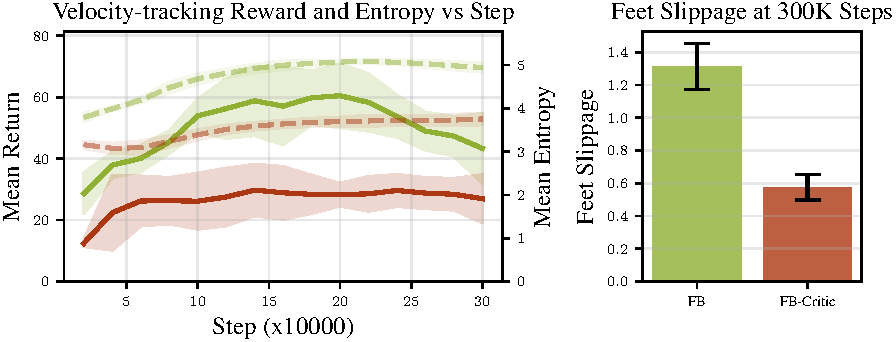
\includegraphics[width=0.8\linewidth]{figure/locomotion_fb_fb_critic.pdf}
   

    % Legend
    \centering
    \minipage{\linewidth}
    \small
    \centering
    \textcolor{ourgreen}{\rule[2pt]{20pt}{3pt}} \textrm{FB} \quad
    \textcolor{ourdarkred}{\rule[2pt]{20pt}{3pt}} \textrm{\algo{FB-Critic}}\quad
    % \textcolor{ourorange}{\hdashrule[2pt]{20pt}{3pt}{2pt 2pt}}\textrm{\algo{dashed example}}
    \endminipage\
    \caption{Limitations of undirected exploration: Standard FB algorithm with undirected exploration (FB) suffers from performance degradation and entropy stagnation (left, higher is better) and yields unnatural behaviors (right, lower is better). While introducing a behavior regularizer (FB-critic) leads to more plausible behaviors (right), it leads to severe performance degradation and further reduces behavior diversity (left).}
    \label{fig:motivation_method}
\end{figure}

\section{Maximum Entropy Behavior Exploration}

\begin{figure}[t]
    \centering
    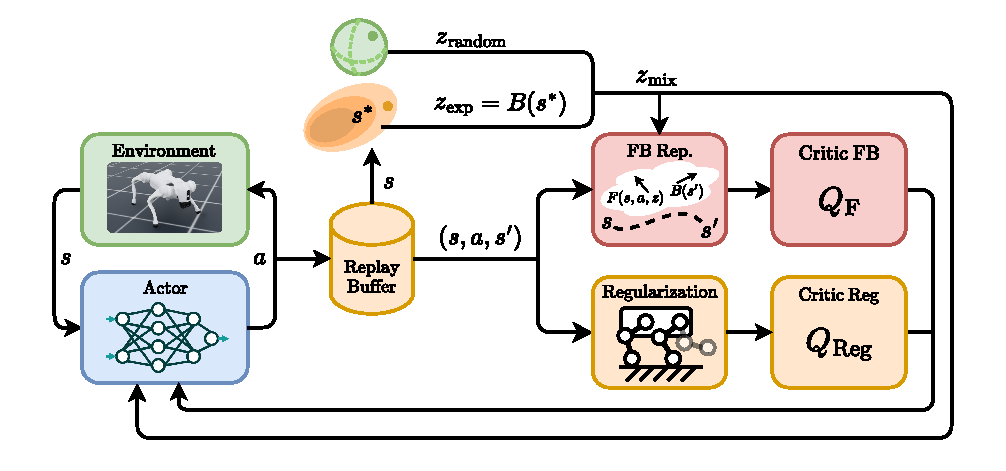
\includegraphics[width=\linewidth]{figure/pipeline.pdf}
    \caption{Maximum Entropy Behavior Forward-Backward Exploration:  \method is an online zero-shot RL algorithm that collects data by acting with behaviors $z_{exp}$ that maximize the entropy of the achieved behavior distribution. Collected data is used to train policies with a regularized loss combining policy improvement objective based on the FB action value function ($Q_{FB}$) and a critic ($Q_{reg}$) trained on a behavior regularizer reward to induce meaningful locomotion patterns.}
    \label{fig:fig_method}
\end{figure}


\subsection{Density-Inverse Exploration for Online FB}


\textit{How should a zero-shot RL agent explore in an environment in order to accumulate diverse, relevant data, while aligned with downstream task of interest?} While we lack a proper characterization of which data is relevant \textit{a priori}, the support of the empirical training distribution $\rho$ must cover the occupancy measures of policies optimal for downstream tasks $z^d_r$. Hence, an exploration strategy should select intrinsic behaviors $z_r^t$ to bring the agent's historical achieved behavior distribution $p^t_{z^a_r}$ close to the downstream behavior distribution $p_{z^d_r}$. This can be formalized with the following distribution matching objective:
\begin{equation}
\label{eq:oracle_loss}
    J_{\text{oracle}}(p^t_{z^a_r}) = D_{KL}(p_{z^d_r} \vert \vert p^t_{z^a_r})
\end{equation}
where $p^t_{z^a_r}$ is the distribution of achieved behaviors in the replay buffer at time $t$ and $D_{KL}$ is the forward KL divergence (support covering).
Unfortunately, in the unsupervised setting, objective in \Cref{eq:oracle_loss} is intractable, because we do not have access to the desired behavior distribution $p_{z^d_r}$. In the absence of a useful inductive bias on the direction where to expand the support of $p_{z^a_r}$, similarly to \citet{pitis2020maximum}, we expand the support on all directions maximizing the entropy of the achieved behavior distribution $H[p^t_{z^a_r}]$. This leads to the following objective:
\begin{equation}
\label{eq:entropy_loss}
    J_{\text{MEBE}}(p^t_{z^a_r}) = -H[p^t_{z^a_r}],
\end{equation}
implicitly inducing a curriculum on the behaviors with which explore next to effectively push the frontier of achievable behaviors. 
% \subsection{Setting intrinsic exploration behaviors}
To optimize \Cref{eq:entropy_loss}, at time $t$ we act with an exploration policy $\pi_t^E$ %which is going to collect data such that the expected entropy of the updated achieved behavior distribution is maximized. Formally, we act with the policy 
with reward embedding $z_r^{E}$ such that
% $z_r^E \sim \nu_{\tiny{\method}}$
\begin{equation}
\label{eq:z_mebe}
    z_r^{E} = \argmax_{z_{r} \in \gZ}\mathbb{E}_{z'_r \sim q(z'_r \vert z_r)} H\big[p^t_{z^a_r \cup z'_r}\big].
\end{equation} 
Importantly, \Cref{eq:z_mebe} depends on $q(z'_r \vert z_r)$ which encodes the conditional probability of achieving behavior $z_r'$ if we act with the policy parameterized with $z_r$, which we do not know. However, we observe that the entropy $H[p^t_{z^a_r}]$ is maximized when the distribution of achieved behaviors is uniform over the behavior space. Consequently, rather than predicting future outcomes, \method steers the achieved behavior distribution towards uniformity by sampling exploration behaviors $z_r^E$ that have the minimum density in the current buffer.%Hence, we select exploration behaviors $z_r^E$ that have minimum density in the current buffer. 

\subsection{Pratical FB-MEBE}
Let $q_\Psi(z^a_r)$ be the density model trained on the achieved behaviors stored in the replay buffer. We sample exploration behaviors according to a distribution that is inversely proportional to their estimated density, i.e., 
\begin{equation}
\label{eq:sample_inv}
   z_r^E \propto ({q}_\psi(z^a_r) + \epsilon)^{-\beta}
\end{equation}
where $\epsilon > 0$ ensures numerical stability and $\beta \ge 0$ controls the strength of the inverse reweighting. 
% This strategy approximates the maximization of the state distribution entropy $H(P(s))$, effectively mitigating occupancy bias during online training.
In practice, because we have direct access to states, we learn the density model on the space of achieved states $q_\Psi(s)$ instead (or on a projection $\varphi(s)$\footnote{To focus exploration on relevant parts of the state space, we learn the density on projections of it i.e., $\varphi: S \rightarrow S'$, where $S\subseteq\sR^d, S' \subseteq \sR^{m}, m<d$.} of it). This effectively focuses on goal-reaching behaviors, i.e., $z_r=B(s)$, and could circumvent challenges arising from representation drifts that occur due to $B$ representations changing through time. 
% An in-depth analysis is left for future work.




 Various approaches can be used to estimate the state density, such as Kernel Density Estimation (KDE), Variational Autoencoders (VAE) \citep{kingma2013auto}, k-NN particle estimators, Random Network Distillation (RND) \citep{rnd} or normalizing flows \citep{rezende2015variational}. We chose normalizing flows (NFs) to fit our density $q_\Psi(s)$ over all the alternatives due to its efficient likelihood evaluation, compared to quadratic computation cost of non-parametric models, while offering true density estimates compared to surrogates produced by RND or VAE. Leveraging NFs for unsupervised goal sampling has been also explored in \citep{normalizing-flow-rl}. Note that during the inverse sampling process, the state $s$ is sampled from the replay buffer rather than from the flow model to improve training stability. Details for the NF can be found in \Cref{tab:nf_hyperparameters}. Finally, we explore with the set of policies with reward embedding
\begin{equation}
\label{eq:practical_fb_mebe}
\{z_j^E = B(s_j^E)\}_{j=1}^K,  \quad s_j^E \sim ({q}^t_\psi(s))^{-\beta}
\end{equation}
where $K$ is the number of exploration policies collecting data in parallel and ${q}^t_\psi(s)$ is the density model fitted on data from the replay buffer at episode $t$. 


Finally, as reported in \Cref{sec:limitations}, \method regularizes exploration by enforcing relevant gait patterns via a behavior regularizer, as in \Cref{eq:actor_loss_with_reg}. 
We provide a pseudocode for our algorithm in \Cref{algo:fb-mebe} and a visual schematic of \method in \Cref{fig:fig_method}. For details, see \Cref{appendix:hyperparams,appendix:qregu}.








\begin{algorithm}
\caption{Maximum entropy behavior exploration (\method)}\label{algo:fb-mebe}
\begin{algorithmic}[1]
    \STATE \textbf{Input:} $F_{\theta}$ and $\bar{F}_{\theta}$, $B_\phi$ and $\bar{B}_{\phi}$, $q_\Psi$, $Q_\mathrm{reg}$ 
    \WHILE{not converged}
        \STATE Sample behavior $z_r^E$ according to \cref{eq:practical_fb_mebe}.
        \STATE Collect data $\gD_n =\mathrm{Rollout}(\pi(z_r^E))$.
        \STATE Add data to buffer $\gD_{1:n} = \gD_{1:n-1} \cup \gD_n$.
        \STATE Fit $F_\theta$, $B_\phi$, policies $\pi_z$, $q_\Psi$ and $Q_\mathrm{reg}$  with $\gD_{1:n}$.
    \ENDWHILE
\end{algorithmic}
\end{algorithm}

%%%%%%%%%%%%%%%%%%%%%%%%%%%%%%%%%%%%%%%%%%%%%%%%%%%%%%%%%%%%%%%%
%% Section: Experiments (Test)
%%%%%%%%%%%%%%%%%%%%%%%%%%%%%%%%%%%%%%%%%%%%%%%%%%%%%%%%%%%%%%%%
\section{Experiments}
Our experiments are designed to address the following questions:
\begin{enumerate}
    \renewcommand{\labelenumi}{\roman{enumi})}
    \item Does \method produce more natural behaviors than unregularized counterparts?
    \item Does \method achieve gains in performance comparing with other exploration strategies? %via efficient exploration
    \item Does \method enable effective transfer from simulation to real-world hardware?
\end{enumerate}
\paragraph{Environment.} All experiments are conducted in IsaacLab simulation environment~\citep{mittal2025isaaclab}. We use the Unitree Go2 quadruped robot with $12$ degrees of freedom. The action space is defined as $\mathcal{A} \subseteq [-1, +1]^{12}$. The simulation runs at $200$\,Hz, while the PD controller operates at $50$\,Hz. Details about state space and domain randomization can be found in \Cref{appendix:observation-space}.

\paragraph{Task Metrics.}
We evaluate \method on two different sets of downstream tasks: velocity-tracking tasks and base orientation tasks. Both the velocity-tracking and base-orientation settings consists of $17$ downstream tasks. Performance is measured by the average episode return achieved on each task, with the episode length equals 250 steps and a maximum achievable reward of $250$. Detailed downstream task reward are in appendix \Cref{appendix:reward-function}. We additionally report the foot sliding to assess locomotion quality (details in \Cref{appendix:regularization_reward}).

\paragraph{Baselines.} We compare \method with several baselines and ablations. FB \citep{touati2021learning} performs undirected exploration by uniformly sampling random reward embeddings from the hypersphere. FB-Critic uses the same uniform exploration strategy as FB but includes our proposed behavior regularizer (see \Cref{sec:limitations}). This isolates the performance gains provided by our exploration strategy from the gains provided by the regularizer. \method ($\beta$=2, our method) includes a behavior regularizer and directs exploration sampling 80\% of its embeddings with our proposed MEBE strategy (\Cref{eq:practical_fb_mebe}) and 20\% using uniform random embeddings. Finally, we include an ablation FB-MEBE ($\beta$=0), which sets the reverse sampling coefficient $\beta$ to zero. This can be seen as an instantiation of FB-CPR \citep{tirinzoni2025zeroshot}, with no data prior. Instead of prioritizing rare behaviors, it performs uniform exploration over the achieved behaviors.  This isolates the performance gains provided by our exploration strategy from the gains provided by the biasing towards goal-reaching behaviors. For other ablations on the $\beta$ parameter and on sampling strategies, see \Cref{appendix:ablation_beta,appendix:ablation_exptrain}, respectively.

In practice, to focus exploration on relevant parts of the state space, we conduct exploration over a lower-dimensional projections of the state rather than directly operating on the full state space. Formally we define a projection mapping $\varphi: S \rightarrow S'$, where $S\subseteq\sR^d, S' \subseteq \sR^{m}, m<d$. For velocity-tracking tasks, exploration is performed in the planar base velocity space $\left[v_x, v_y\right]$. For base-orientation tasks exploration is performed in the space of the gravity vector expressed in the robot base frame $\left[g_x, g_y, g_z\right]$, which characterizes the base orientation. While this restricts the exploration scop to task-relevant settings, \method could be easily extended to operate directly on the full state-space, which we leave for future work.  

% \todo{Add the Vxy filtering in appendix, maybe later use FB-MEBE without filtering so we don't need to introduce filtering}

\subsection{Main Results}
\begin{figure}[H]
    \centering
    \begin{minipage}{\textwidth}
    \centering
    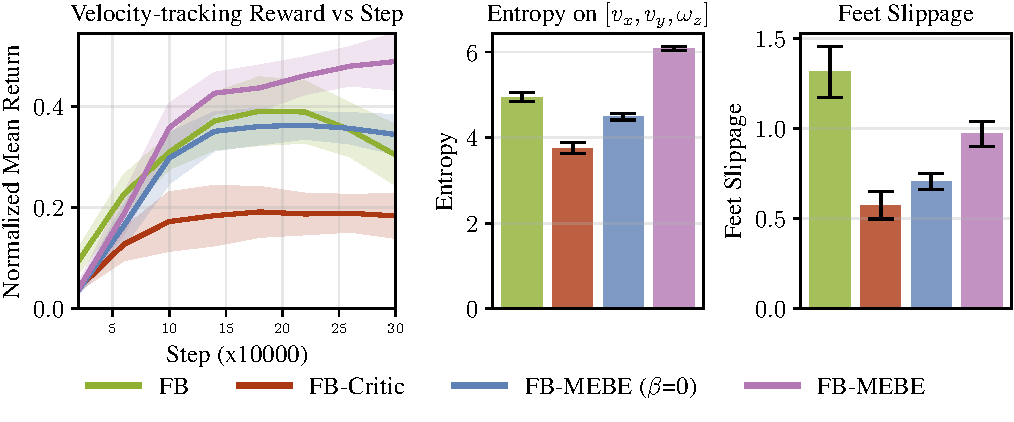
\includegraphics[width=0.8\linewidth]{figure/locomotion_list_mean_fast_td3_exp_and_train.pdf}
    \end{minipage}
% \end{figure}

% \begin{figure}[H]
    \begin{minipage}{\textwidth}
    \centering
    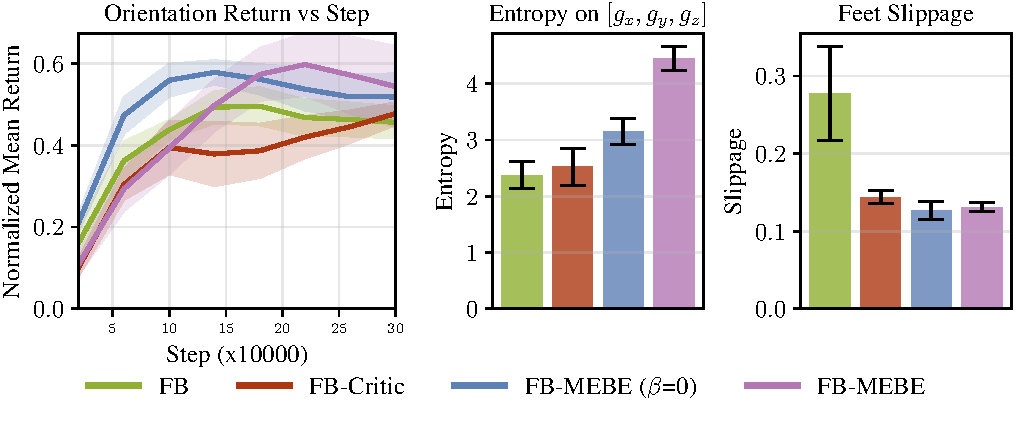
\includegraphics[width=0.8\linewidth]{figure/orientation_list_mean_fast_td3_exp_and_train.pdf}
    \end{minipage}
    \caption{
    Left: Zero-shot performance averaged over 17 downstream velocity tracking tasks (top) and orientation tasks (bottom). We plot normalized return wrt the mean return of Fast-TD3 \citep{seo-2025}. 
    Results are averaged across 5 random seeds, with shaded regions indicating $\pm$ 1-standard deviation. 
    Middle: Policy entropy on $\left[v_x, v_y, w_z \right]$ (top)  and $\left[g_x, g_y, g_z\right]$ (bottom) measured at 300K training steps. (Higher is better). 
    Right: Feet slippage measured at 300K training steps. (Lower is better).}
    \label{fig:FB-MEBE}
\end{figure}

\paragraph{Overall Performance.}
In \Cref{fig:FB-MEBE}, we report results on several downstream tasks. All returns are normalized using the mean return achieved by Fast-TD3 \citep{seo-2025}. Fast-TD3 is a supervised reinforcement learning algorithm trained directly with task-specific rewards, and therefore serves as an approximate upper bound under explicit reward supervision. In contrast, all FB-based methods are trained without access to downstream task rewards and must rely on unsupervised exploration to acquire useful behaviors. %As a result, their performance is naturally lower than that of Fast-TD3.
 \method achieves an average performance that is the highest over all the other baselines for velocity tracking tasks or on par with best performing baseline for orientation tasks. Most notably, it yields the highest entropy among all baselines. This indicates that \method expands behavioral coverage during online training. Importantly, this broader exploration translates into improved downstream task performance rather than unstructured behavior diversification. This can be further seen in \Cref{fig:FB-MEBE-Detailed-Perforance,fig:orientation} where \method outperforms all other baselines in extreme downstream tasks. For orientation tasks, \method shows lower sample efficiency than \method-$\beta=0$, showcasing that unprioritized goal-reaching exploration can be a valid strategy for some downstream tasks. In contrast, FB and FB Critic performs the worst among all algorithms, which we attribute to uninformed exploration (FB) and the additional regularization constraints (FB-critic) that overly restrict exploration, specially in velocity-tracking tasks, leading to limited behavioral coverage and consequently lower average performance.  Regarding gait-related metrics, FB-MEBE substantially reduces the feet slide penalty compared to the original FB, indicating that the regularization critic successfully suppresses unnatural dragging behaviors. Although FB-MEBE exhibits slightly higher feet slippage than FB-Critic, this difference is expected. Since FB-MEBE actively explores higher locomotion velocities, increased horizontal foot velocities naturally lead to higher sliding penalties. Therefore, the observed difference reflects expanded behavioral coverage rather than degraded gait stability. %Overall, FB-MEBE achieves a better balance between exploration capacity and task performance.

%%%%%%%%%%%%%%%%%%%%%%%%%%%%%%%%%%%
\paragraph{Detailed Locomotion Performance.}
\Cref{fig:FB-MEBE-Detailed-Perforance} reports performance across 17 velocity-tracking tasks. 
For moderate velocity commands, all methods obtain reasonable returns. However, for high-velocity tasks, all baselines suffer noticeable performance degradation. This phenomenon is consistent with the replay buffer distribution shown in \Cref{appendix:replay_buffer_data_distribution}, where naive online FB training (FB baseline) progressively concentrates data in low-velocity regions. This distributional shrinkage leads to insufficient coverage of high-speed behaviors and limits zero-shot performance to boundary velocity tasks. By contrast, FB-MEBE expands the replay buffer coverage tencouraging exploration in sparsely visited velocity regions. Consequently, FB-MEBE maintains strong performance even on boundary tasks, demonstrating improved downstream performance.

\begin{figure}[H]
    \centering
    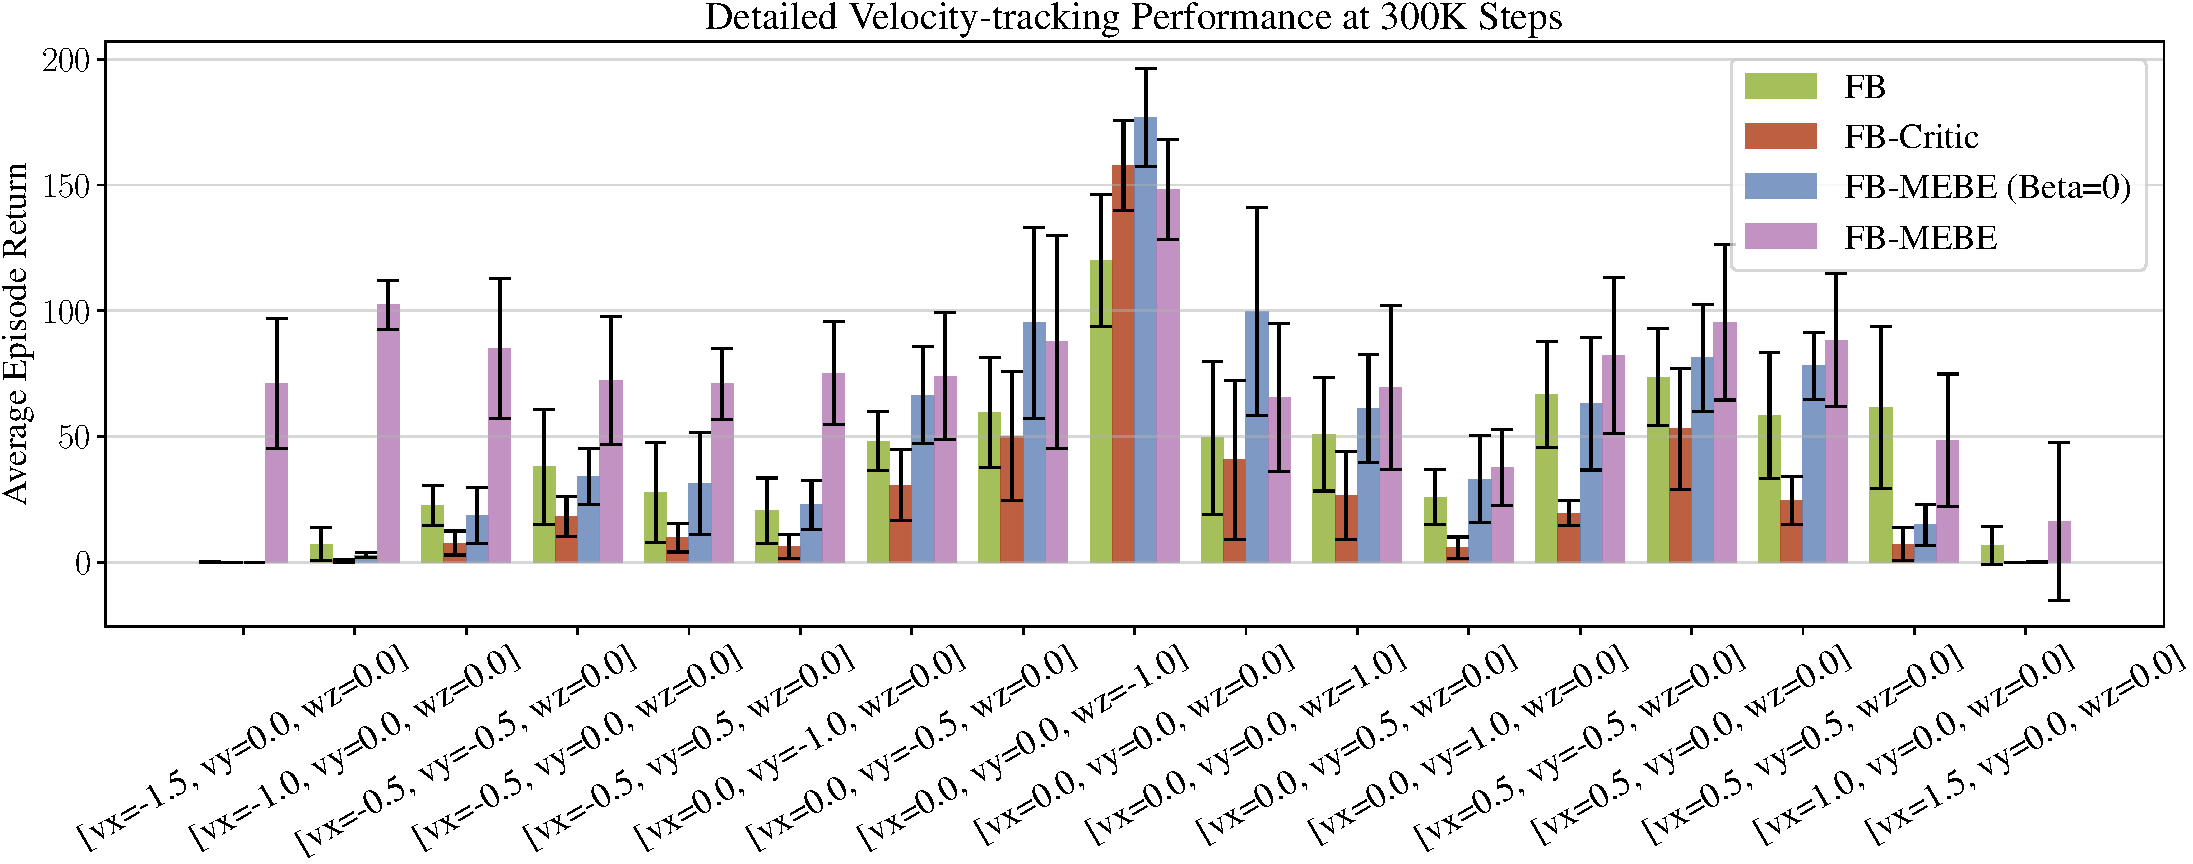
\includegraphics[width=1.0\linewidth]{figure/comparison_detailed_locomotion_task_exp_and_train.pdf}
    \caption{
    Comparison of different methods under detailed locomotion command settings. 
    Each group on the x-axis corresponds to a target velocity command $[v_x, v_y, \omega_z]$. 
    The y-axis reports the mean episode return evaluated under the reward function (in \Cref{appendix:reward-function}) associated with the corresponding target velocity. 
    Results are averaged over 5 random seeds, and error bars denote $\pm$ 1-standard deviation.
    }
    \label{fig:FB-MEBE-Detailed-Perforance}
\end{figure}
\paragraph{Detailed Orientation Performance.}
\Cref{fig:orientation} shows the performance across 12 base orientation tracking settings. 
Notably, \method demonstrates superior performance on challenging large-angle tasks compared to baselines. This indicates enhanced exploration within the orientation behavior space.
However, we observe that FB-MEBE achieves lower returns than baselines on small-angle orientation tasks, including FB-critic (which could be due to the behavior regularization not impeding exploration for orientation tasks). This suggests that \method allocates more model capacity towards extreme behaviors. Balancing this capacity, could be addressed through further finetuning of the exploration ratio.
\begin{figure}[t]
    \centering
    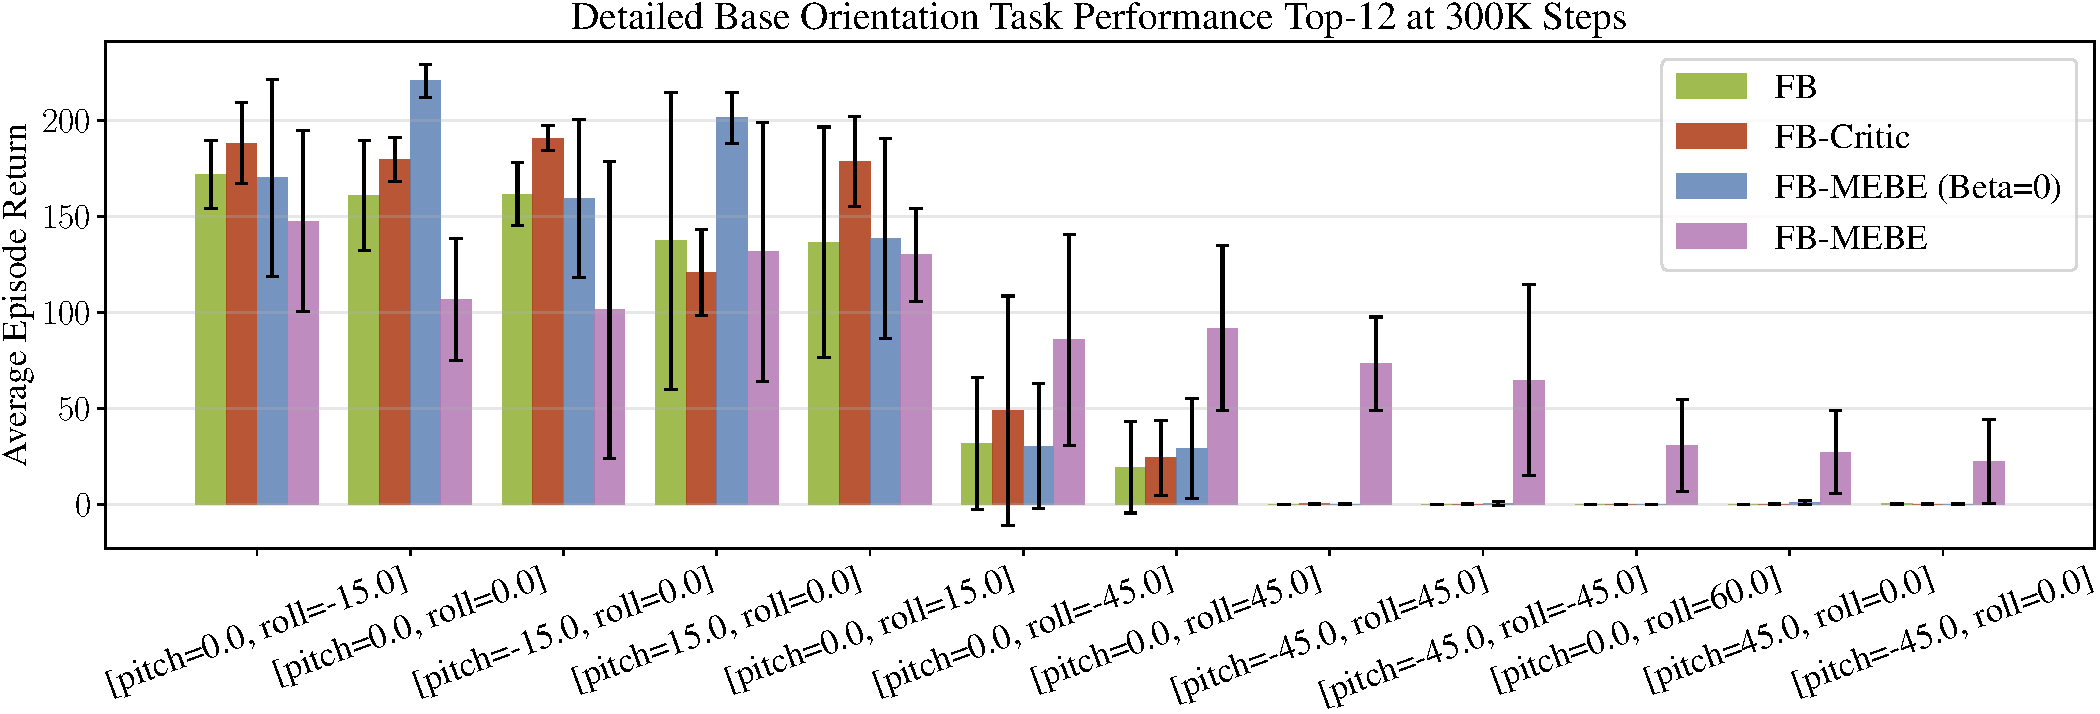
\includegraphics[width=1.0\linewidth]{figure/comparison_detailed_orientation_task_exp_and_train.pdf}
    \caption{
    Comparison of different methods under detailed orientation command settings. Each group on the x-axis corresponds to a target orientation command $[\text{Pitch}, \text{Roll}]$. We removed tasks for which all algorithms get rewards smaller than one from the graph.
    % The y-axis reports the mean episode return evaluated under the reward function (in \Cref{appendix:reward-function}) associated with the corresponding target orientation. 
    % Results are averaged over 5 random seeds, and error bars denote $\pm$ 1-standard deviation. 
    }    
    \label{fig:orientation}
\end{figure}

%%%%%%%%%%%%%%%%%%%%%%%%%%%%%%%%%%%


\paragraph{Hardware Tests.}
We deploy FB-MEBE on a real Unitree Go2 robot and evaluate it on both locomotion and orientation control tasks. To facilitate real-world control, commands are issued through a joystick interface, and the robot is guided by a composite reward function (details in \Cref{appendix:reward-function}) that simultaneously regulates velocity, base orientation, and base height. 

As illustrated in \Cref{fig:sim2real}, FB-MEBE enables the robot to track commanded translational velocities, adjust pitch and roll orientations, and regulate its height. The learned policy also supports compositional commands, such as walking forward while maintaining a pitch angle of $15^\circ$, or tracking yaw angular velocity while keeping the base height at $0.32\,\mathrm{m}$. 

Importantly, the resulting behaviors remain stable and natural, without exhibiting excessive action rates or noticeable foot slippage that could destabilize the robot.

\begin{figure}[H]
    \centering
    \begin{minipage}[b]{0.25\linewidth}
        \centering
        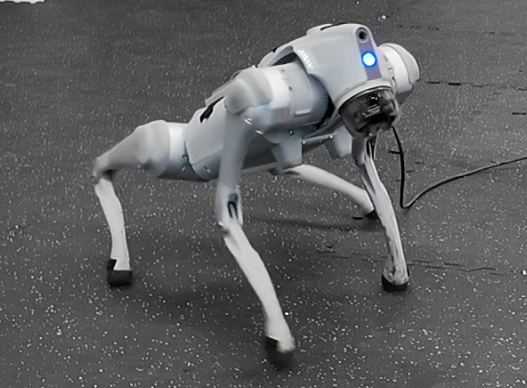
\includegraphics[width=\linewidth]{figure/sim2real_pitch_up.png}
    \end{minipage}
    \begin{minipage}[b]{0.25\linewidth}
        \centering
        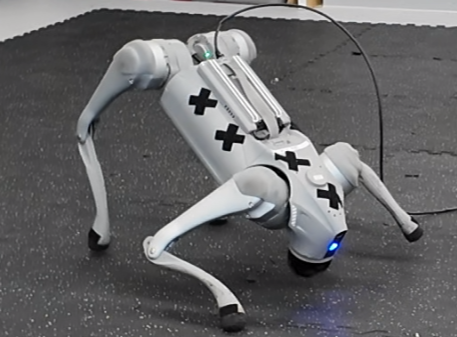
\includegraphics[width=\linewidth]{figure/sim2real_pitch_down.png}
    \end{minipage}
    \begin{minipage}[b]{0.25\linewidth}
        \centering
        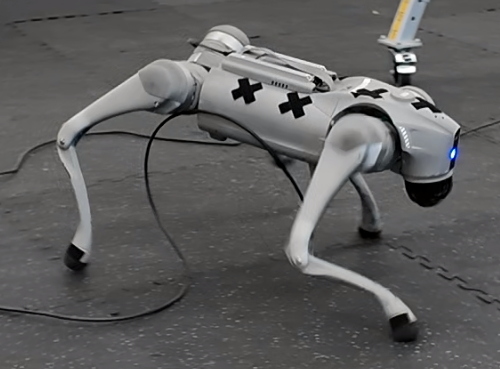
\includegraphics[width=\linewidth]{figure/sim2real_forward.png}
    \end{minipage}
    \caption{\method allows for zero-shot sim2real transfer to Unitree Go2, a commercial quadrupedal robot. }
    \label{fig:sim2real}
\end{figure}
\section{Conclusion}
We propose \method, a practical online zero-shot RL algorithm that enables efficient exploration for learning quadrupedal control. \method addresses the undirected exploration of naive online FB algorithm, by using an exploration strategy that guides data collection policies towards maximizing the entropy of the achieved behavior distribution. To constrain exploration, \method introduces a behavior regularizer, shaping the recovered policies towards more natural and physically plausible patterns. Through this novel yet simple approach, \method yields policies that can be seamlessly deployed to hardware without further finetuning. To the best of our knowledge, this is the first instantiation of  fully online zero-shot RL algorithm on real robotics systems without relying on external datasets as motion priors.

While \method represents a principled attempt toward efficient online zero-shot RL, some limitations remain. The recovered policies will struggle with downstream tasks requiring behaviors that fall far outside from the collected dataset. Additionally, the exploration strategy is still loosely constrained, which can occasionally lead the agent to explore extreme state configurations that are irrelevant for downstream task of interest. A deeper theoretical understanding of the FB algorithm's components could provide better intuition regarding whether FB implicitly prioritizes some behaviors over than others. Finally, while we leveraged a useful behavior regularizer, developing more theoretically sound ways to characterize a specific family of reward functions of interest could lead to safer, more directed exploration in future work.


\subsubsection*{Broader Impact Statement}
\label{sec:broaderImpact}
% \nuria{In this optional section, RLJ/RLC encourages authors to discuss possible repercussions of their work, notably any potential negative impact that a user of this research should be aware of. }
Our work focuses on zero-shot RL algorithms for quadrupedal control. While we recognize that autonomous robotic systems have the potential to be deployed for harmful applications, our contributions are fundamental in nature and do not directly target any specific negative use cases.

%%%%%%%%%%%%%%%%%%%%%%%%%%%%%%%%%%%%%%%%%%%%%%%%%%%%%%%%%%%%%%%%
%% Appendices
%%%%%%%%%%%%%%%%%%%%%%%%%%%%%%%%%%%%%%%%%%%%%%%%%%%%%%%%%%%%%%%%
\appendix

% \section{The first appendix}
% \label{sec:appendix1}
% This is an example of an appendix. 

% \noindent \textbf{Note:} Appendices appear before the references and are viewed as part of the ``main text'' and are subject to the 8--12 page limit, are peer reviewed, and can contain content central to the claims of the paper. 

% \section{The second appendix}
% \label{sec:appendix2}
% This is an example of a second appendix. If there is only a single section in the appendix, you may simply call it ``Appendix'' as follows:

% \input{Appendix}

\subsubsection*{Acknowledgments}
\label{sec:ack}
The authors thank Marco Bagatella and Thomas Rupf for their valuable feedback and for helping reviewing the manuscript.
Núria Armengol is supported by the Max Planck ETH Center for Learning Systems.


%%%%%%%%%%%%%%%%%%%%%%%%%%%%%%%%%%%%%%%%%%%%%%%%%%%%%%%%%%%%%%%%
%% NOTE: THIS MARKS THE END OF THE "MAIN TEXT"
%%%%%%%%%%%%%%%%%%%%%%%%%%%%%%%%%%%%%%%%%%%%%%%%%%%%%%%%%%%%%%%%

%%%%%%%%%%%%%%%%%%%%%%%%%%%%%%%%%%%%%%%%%%%%%%%%%%%%%%%%%%%%%%%%
%% Bibliography
%%%%%%%%%%%%%%%%%%%%%%%%%%%%%%%%%%%%%%%%%%%%%%%%%%%%%%%%%%%%%%%%
\bibliography{main}
\bibliographystyle{rlj}

%%%%%%%%%%%%%%%%%%%%%%%%%%%%%%%%%%%%%%%%%%%%%%%%%%%%%%%%%%%%%%%%
% AUTHOR: If your paper has no supplementary materials, you may 
%         comment out the line below, which creates the title for
%         the supplementary materials.
%%%%%%%%%%%%%%%%%%%%%%%%%%%%%%%%%%%%%%%%%%%%%%%%%%%%%%%%%%%%%%%%
\beginSupplementaryMaterials

%%%%%%%%%%%%%%%%%%%%%%%%%%%%%%%%%%%%%%%%%%%%%%%%%%%%%%%%%%%%%%%%%%%%%%%%%%%%%%%%%%%%%%%%%%%%%%%%%%%%%%%%%%%%%%
\section{Algorithm Details}
\label{app:fb_algo_details}
Following prior work on Forward-Backward (FB) representations \citep{touati2023does}, we include two additional regularization losses to stabilize FB training. First, we adopt an orthonormality regularization on the backward representation $
\Sigma_B = \mathbb{E}\left[B(s)B(s)^\top\right]$,
which encourages the covariance of $B(s)$ to approach the identity matrix. This regularization prevents the backward representation from collapsing and improves the conditioning of the learned embedding space. Second, we introduce a temporal-difference regularization loss on the forward map that encourages $
F(s,a,z)^\top z
$ to approximate the action-value function corresponding to the reward induced by $B(s)^\top \Sigma_B^{-1}z$. This loss encourages the forward representation to capture directions in the latent space that are relevant for policy optimization. See \citep{touati2023does} (Appendix B) for more details.

%%%%%%%%%%%%%%%%%%%%%%%%%%%%%%%%%%%%%%%%%%%%%%%%%%%%%%%%%%%%%%%%%%%%%%%%%%%%%%%%%%%%%%%%%%%%%%%%%%%%%%%%%%%%%%

% \section{Prior Information on Rewards}
% \todo{unfinished}
% $\phi(s,a) = [v, \omega,g,h]$ where $v$ is the 3-dimension base linear velocity, $\omega$ is the 3-dimension base angular velocity, $g$ is the 3-dimension base gravity vector and h is 1-dimension base height. 

%%%%%%%%%%%%%%%%%%%%%%%%%%%%%%%%%%%%%%%%%%%%%%%%%%%%%%%%%%%%%%%%%%%%%%%%%%%%%%%%%%%%%%%%%%%%%%%%%%%%%%%%%%%%%%
\section{Practical Exploration}
\label{appendix:practical-exploration}
To improve exploration efficiency in this setting, we discard states where the robot pitch or roll exceeds $21.5^\circ$. These states typically correspond to failure events such as falling, which can produce large velocities unrelated to meaningful locomotion behaviors. Filtering such degenerate transitions helps focus exploration on valid locomotion regimes.
%%%%%%%%%%%%%%%%%%%%%%%%%%%%%%%%%%%%%%%%%%%%%%%%%%%%%%%%%%%%%%%%%%%%%%%%%%%%%%%%%%%%%%%%%%%%%%%%%%%%%%%%%%%%%%

\section{Ablation Tests}
\subsection{Ablation Study on $\beta$.} 
\label{appendix:ablation_beta}
\Cref{fig:Abalation} presents the ablation results with different inverse-density coefficients $\beta$. When $\beta=0$, corresponding to uniform latent sampling without density reweighting, both entropy and task reward remain relatively low. As $\beta$ increases, entropy and reward consistently improve.

These results confirm that inverse-density reweighting effectively increases the entropy of the achieved behavior distribution and mitigates replay buffer occupancy collapse during online training.

% \begin{figure}[H]
%     \centering
%     \includegraphics[width=0.6\linewidth]{figure/experiments_ablation_2.png}
%     \caption{Comparison between different betas}
%     \label{fig:placeholder}
% \end{figure}

\begin{figure}[H]
    \centering
    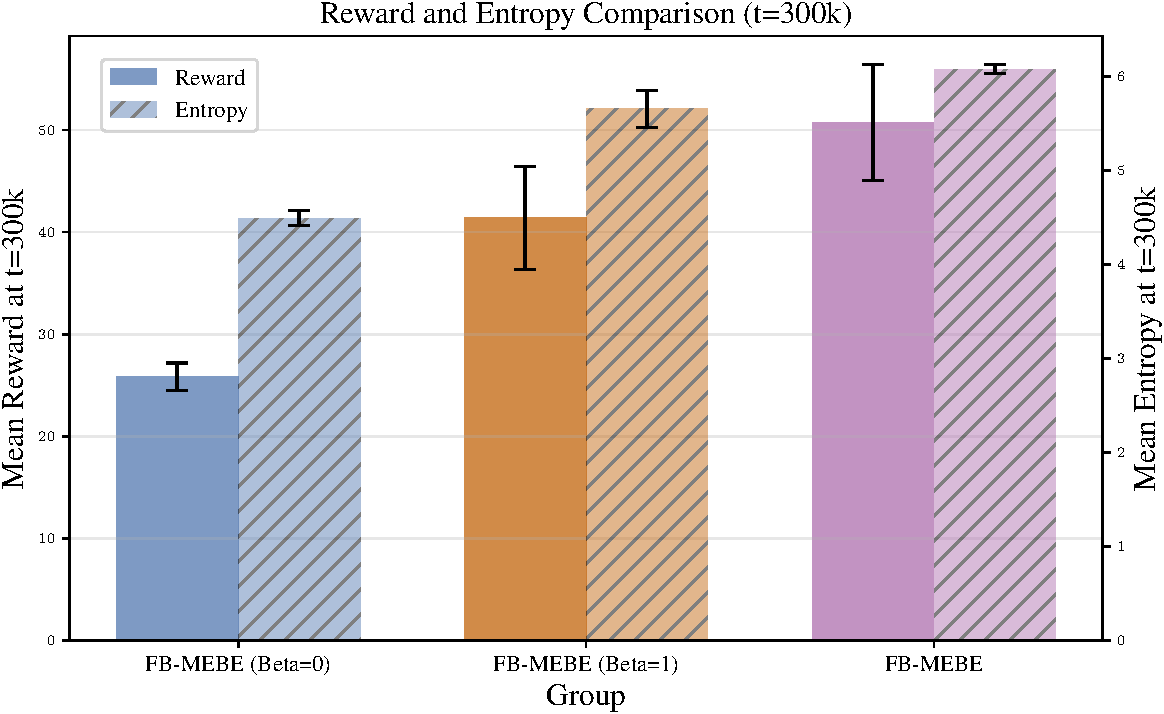
\includegraphics[width=0.6\linewidth]{figure/fb-mebe-comparison-beta.pdf}
    \caption{Comparison between different betas on FB-MEBE on locomotion tasks}
    \label{fig:Abalation}
\end{figure}
\subsection{Ablation study on sampling strategy}
\label{appendix:ablation_exptrain}
We evaluate a version of \method (\method-\text{abl}), that performs an ablation on the sampling strategy used for \textit{training} the FB representations.
\method uses the \textit{same} sampling strategy for reward embeddings used for data collection ($0.8 z_{exp}$ + $0.2 z_{random}$) and the reward embedding used for training FB representations.
Here, we compare with an alternative version which only uses our  strategy for data collection, and uses $(0.8 z_\text{goal reaching} + 0.2 z_\text{random}$ for training. The later is analogous to the exploration strategy $\method(\beta=0)$ uses.
While \method puts more emphasis on learning FB representations and policies for low visitation behaviors and might hence learn better policies useful for exploration,\method-\text{abl} samples exploration behaviors uniformly from the replay buffer.
While these two approaches are different in nature, in practice we do not find significant differences as can be seen in \Cref{fig:ablation_exptrain1}. Extensive evaluation on different mixing ratios can also bring more insights on better sampling alternatives.


% TEMP
\begin{figure}
    \centering
    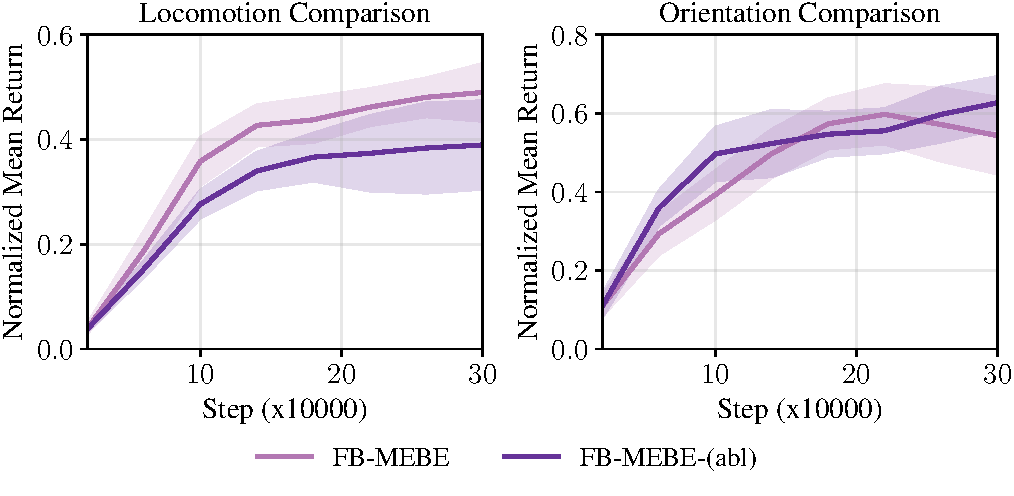
\includegraphics[width=0.8\linewidth]{figure/compare_exp_with_exp_and_train.pdf}
    \caption{Comparison on velocity-tracking tasks between \method and an ablation \method-\text{abl} leveraging different sampling strategies for training the FB algorithm}
    \label{fig:ablation_exptrain1}
\end{figure}


%%%%%%%%%%%%%%%%%%%%%%%%%%%%%%%%%%%%%%%%%%%%%%%%%%%%%%%%%%%%%%%%%%%%%%%%%%%%%%%%%%%%%%%%%%%%%%%%%%%%%%%%%%%%%%
\section{Replay buffer data distribution}
\label{appendix:replay_buffer_data_distribution}
\begin{figure}[H]
    \centering
    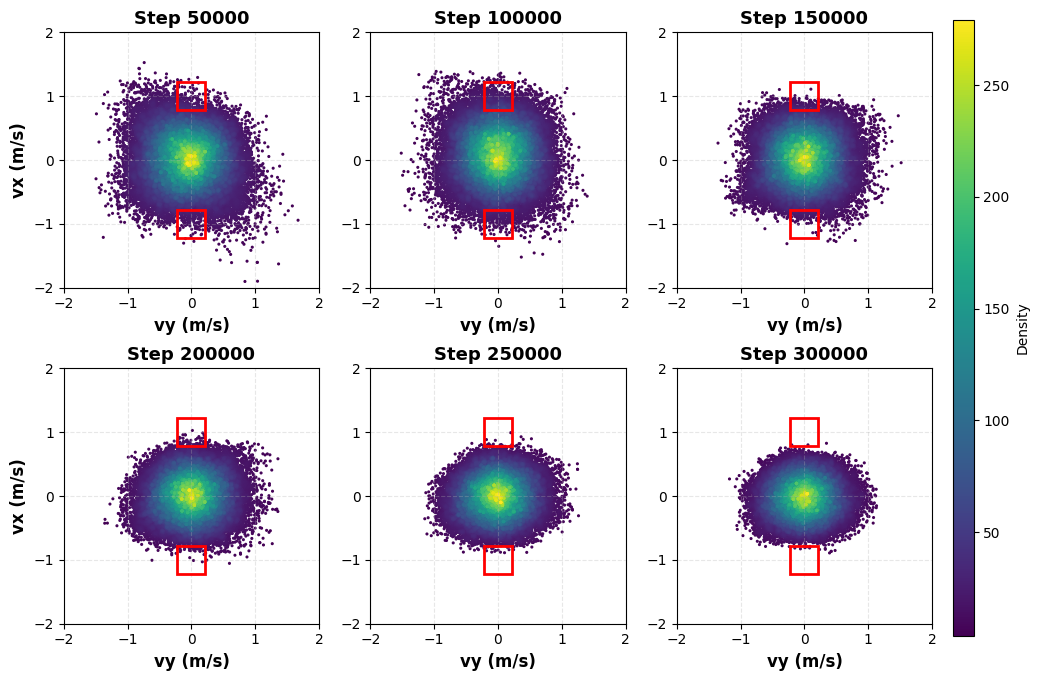
\includegraphics[width=0.8\linewidth]{figure/Appendix_FB_buffer_change.png}
    \caption{Velocity $\left[v_x, v_y \right]$ distribution of FB replay buffer at different training step. The color represents the density of data points.}
    \label{fig:replay_buffer_data_distribution}
\end{figure}


%%%%%%%%%%%%%%%%%%%%%%%%%%%%%%%%%%%%%%%%%%%%%%%%%%%%%%%%%%%%%%%%%%%%%%%%%%%%%%%%%%%%%%%%%%%%%%%%%%%%%%%%%%%%%%
\section{Task Reward Function}
\label{appendix:reward-function}

 Let $\mathbf{v} \in \mathbb{R}^3$ and $\boldsymbol{\omega}_z \in \mathbb{R}$ denote the current base linear velocity and yaw angular velocity, respectively,  $h \in \mathbb{R}$ denote the current base height and let $\mathbf{g} \in \mathbb{R}^3$ denote the projected gravity vector. The corresponding command targets are denoted by $\mathbf{v}^\ast$, $\omega_z^\ast$,  $h^*$, and $\mathbf{g}^\ast$.\\
\\
We define the tracking errors as
\begin{align}
e_v &= \lVert \mathbf{v} - \mathbf{v}^\ast \rVert_2, \\
e_\omega &= \lvert \omega_z - \omega_z^\ast \rvert, \\
e_g &= \lVert \mathbf{g} - \mathbf{g}^\ast \rVert_2 \\
e_h &=  \lVert h - h^\ast \rVert_2.
\end{align}
\\
The individual reward terms are computed using Gaussian-shaped functions:
\begin{align}
r_v &= \exp\left(-\left(\frac{e_v}{0.3}\right)^2\right), \\
r_\omega &= \exp\left(-\left(\frac{e_\omega}{0.2}\right)^2\right), \\
r_g &= \exp\left(-\left(\frac{e_g}{0.1}\right)^2\right), \\
r_h &= \exp\left(-\left(\frac{e_h}{0.05}\right)^2\right).
\end{align}
\\

The locomotion and orientation task reward is defined as follows:

\begin{align}
r_{\text{locomotion}} &= r_v \cdot r_\omega \cdot r_g \\
r_{\text{orientation}} &= r_g \cdot r_h
\end{align}

The reward for sim-to-real transfer is defined by multiplication of all terms:
\begin{equation}
r_{\text{sim2real}} = r_v \cdot r_\omega \cdot r_g \cdot r_h
\end{equation}

%%%%%%%%%%%%%%%%%%%%%%%%%%%%%%%%%%%%%%%%%%%%%%%%%%%%%%%%%%%%%%%%%%%%%%%%%%%%%%%%%%%%%%%%%%%%%%%%%%%%%%%%%%%%%%
\section{Regularization rewards}
\label{appendix:regularization_reward}

We provide the mathematical definitions of the regularization reward.  Let $N_j$ denote the number of actuated joints and $N_f$ the number of feet. At time step $t$, let $\ddot{\mathbf{q}}_t \in \mathbb{R}^{N_j}$ be the joint acceleration vector, $\mathbf{a}_t \in \mathbb{R}^{N_j}$ be the action vector, and $\mathbf{a}_{t-1}$ be the previous action.  For each foot $i \in \{1,\dots,N_f\}$, let $h_{t,i}$ be its vertical position (world frame), and $\mathbf{v}^{xy}_{i,t} \in \mathbb{R}^{2}$ be its horizontal linear velocity (world frame). \\

\paragraph{Joint acceleration penalty.}
The joint-acceleration penalty is defined as the squared $\ell_2$ norm of the joint acceleration vector:
\begin{equation}
r_{\text{joint\_acc}}
=
\|\ddot{\mathbf{q}}_t\|_2^2
=
\sum_{k=1}^{N_j} \left(\ddot{q}_{t,k}\right)^2 .
\end{equation}

\paragraph{Action rate penalty.}
The action-rate penalty discourages abrupt changes between consecutive actions:
\begin{equation}
r_{\text{action\_rate}}
=
\|\mathbf{a}_t - \mathbf{a}_{t-1}\|_2^2
=
\sum_{k=1}^{N_j} \left(a_{t,k}-a_{t-1,k}\right)^2 .
\end{equation}

\paragraph{Feet slippage.}
The feet-slide penalty penalizes horizontal foot motion during ground contact.
A binary contact indicator $c_{t,i}$ is defined as
\begin{equation}
c_{t,i}
=
\begin{cases}
1, & \text{if } h_{t,i} > h_{\mathrm{feet\_contact}}, \\
0, & \text{otherwise}.
\end{cases}
\end{equation}

\begin{equation}
r_{\mathrm{feet\_slide}}
=
\sum_{i=1}^{N_f}
c_{t,i}
\,
\|\mathbf{v}_{t,i}^{xy}\|_2 .
\end{equation}

% \paragraph{Feet air-time reward.}
% Let $c_{i,t}\in\{0,1\}$ be an indicator of \emph{first contact} for foot $i$ at step $t$ (i.e., $c_{i,t}=1$ iff the foot transitions from air to contact),
% and let $T^{\text{air}}_{i,t}\ge 0$ be the \emph{last air time} accumulated for foot $i$ before this contact.
% Given a threshold $\tau = 0.5$, the air-time reward is:
% \begin{equation}
% r_{\text{air}} \;=\; \sum_{i=1}^{N_f} \left(T^{\text{air}}_{i,t}-\tau\right)\, c_{i,t}.
% \end{equation}

% \paragraph{Feet clearance reward.}
% Given a target clearance height $h^\star = 0.1$, a scale parameter $\sigma = 0.005$ (named \texttt{std} in code),
% and $\kappa = 2.0$ (named \texttt{tanh\_mult}), we define for each foot:
% \begin{equation}
% e_{i,t}
% \;=\;
% \left(h_{i,t}-h^\star\right)^2
% \;\cdot\;
% \tanh\!\Big(\kappa \, \left\|\mathbf{v}^{xy}_{i,t}\right\|_2\Big),
% % \end{equation}
% and the clearance reward is computed as:
% \begin{equation}
% r_{\text{clearance}}
% \;=\;
% \exp\!\left(
% -\frac{\sum_{i=1}^{N_f} e_{i,t}}{\sigma}
% \right).
% \end{equation}

\paragraph{Total typical regularization reward.}
In our experiments, the regularization reward used to train the critic is:
\begin{equation}
r_{\text{reg}} =
-2.5\times 10^{-7}\, r_{\text{joint\_acc}}
-0.1\, r_{\text{action\_rate}}
-0.1\, r_{\text{feet\_slide}}
\end{equation}


\section{Regularized Exploration.}
\label{appendix:qregu}
We use critic $Q_{\text{reg}}(s,a)$ to estimate the long-term return of the barrier regularization reward $r_{\text{reg}}$ defined in \Cref{appendix:regularization_reward}. Given tuples $(s,a,r_{\text{reg}},s')$ sampled from the replay buffer, we train the regularization critic by minimizing a standard temporal-difference (TD) loss:
\begin{equation}
\mathcal{L}_{\text{critic}}(Q_\text{reg})
=
\mathbb{E}_{ (s,a,s')\sim \rho,a'\sim\pi_z (s')}\Big[
\big(
Q_{\text{reg}}(s,a)
-
\big(r_{\text{reg}}
+
\gamma \,
\bar Q_{\text{reg}}(s', a')
\big)
\big)^2
\Big]
\label{eq:reg_critic_loss}
\end{equation}
\\
Therefore, to pretrain FB agent and learn good gait at the same time, we have the following actor loss:
\begin{equation}
\mathcal{L}_{\text{actor}}(\pi)
=
-\mathbb{E}_{z\sim\nu,\; s\sim\rho,\; a\sim\pi_z(s)}\Big[
Q_{\text{FB}}(s,a,z)
+
\lambda_{\text{reg}}\,
Q_{\text{reg}}(s,a)
\Big]
% \label{eq:actor_loss_with_reg}
\end{equation}

%%%%%%%%%%%%%%%%%%%%%%%%%%%%%%%%%%%%%%%%%%%%%%%%%%%%%%%%%%%%%%%%%%%%%%%%%%%%%%
\newpage % split page temporarily (will delete later)
\section{Simulation Setup}

\paragraph{Joint Control}
We employ joint position control as the low-level control interface. The joint configuration of the robot in the standing pose is defined as the nominal joint position $q_{nom}$. The policy outputs joint position offsets $a$, which are scaled by a factor $s$ and added to the nominal configuration to obtain the target joint positions
\begin{equation}
q_{target} = q_{nom} + s \cdot a .
\end{equation}
The target joint positions are tracked using a PD controller
\begin{equation}
\tau = K_p (q_{target} - q) + K_d (\dot{q}_{target} - \dot{q}),
\end{equation}
where $q$ and $\dot q$ denote the current joint positions and velocities.

\begin{table}[H]
\centering

\begin{minipage}[t]{0.48\textwidth}
\centering
\caption{Joint Control Parameters}
\vspace{0pt}
\begin{tabular}{l c}
\toprule
\textbf{Parameter} & \textbf{Value} \\
\midrule
Action Scale 
    & $0.5$ \\
Proportional Gain $K_p$ 
    & $25.0$\\
Derivative Gain $K_d$ 
    & $0.5$\\
Control Frequency [Hz] 
    & $50\text{Hz}$\\
\bottomrule
\end{tabular}

\end{minipage}
\end{table}

\paragraph{Domain Randomization and Observation Noise}
\begin{table}[H]
\centering

\begin{minipage}[t]{0.48\textwidth}
\centering
\caption{Domain Randomization}
\vspace{0pt}
\begin{tabular}{l c}
\toprule
\textbf{Parameter} & \textbf{Range} \\
\midrule
Friction Coefficient 
    & $\mathcal{U}([0.5,\,1.5])$ \\
Base COM Offset [m] 
    & $\mathcal{U}([-0.05,\,0.05])$ \\
Base Mass perturbation [kg]
    & $\mathcal{U}([-2.0,\,2.0])$ \\
Link Mass Offset [m] 
    & $\mathcal{U}([-0.01,\,0.01])$ \\
Link Mass perturbation [kg]
    & $\mathcal{U}([-0.2,\,0.2])$ \\
Default Joint Pos [rad] 
    & $\mathcal{U}([-0.3,\,0.3])$ \\
\bottomrule
\end{tabular}
\end{minipage}
\hfill
\begin{minipage}[t]{0.48\textwidth}
\centering
\caption{Additive Observation Noise}
\vspace{0pt}
\begin{tabular}{l c}
\toprule
\textbf{Observation} & \textbf{Range} \\
\midrule
$v$ [m/s] 
    & $\mathcal{U}([-0.1,\,0.1])$ \\
$\omega$ [rad/s] 
    & $\mathcal{U}([-0.2,\,0.2])$ \\
$\mathrm{grav}$ 
    & $\mathcal{U}([-0.05,\,0.05])$ \\
$q$ [rad] 
    & $\mathcal{U}([-0.01,\,0.01])$ \\
$\dot{q}$ [rad/s] 
    & $\mathcal{U}([-0.15,\,0.15])$ \\
\bottomrule
\end{tabular}
\end{minipage}

\end{table}

%%%%%%%%%%%%%%%%%%%%%%%%%%%%%%%%%%%%%%%%%%%%%%%%%%%%%%%%%%%%%%%


\section{Observation Space}
\label{appendix:observation-space}
\begin{table}[H]
  \centering
  \renewcommand{\arraystretch}{1.15}
  \begin{tabular}{l l}
    \toprule
    Network & Obs Dimension Breakdown\\
    \midrule

    Critic $(F)$ 
    & $ \left[ \mathbf{v}_{3}, \boldsymbol{\omega}_{3}, \mathbf{g}_{3}, h_{\text{base},1}, \mathbf{q}_{12}, \dot{\mathbf{q}}_{12} \right]$ \\

    $B$ 
    & $ \left[ \mathbf{v}_{3}, \boldsymbol{\omega}_{3}, \mathbf{g}_{3}, h_{\text{base},1} \right]$ \\

    Actor
    & $ \left[ \mathbf{v}_{3}, \boldsymbol{\omega}_{3}, \mathbf{g}_{3}, \mathbf{q}_{12}, \dot{\mathbf{q}}_{12}, \mathbf{a}_{12} \right]$ \\

    Critic (Reg)
    & $\left[ \mathbf{v}_{3}, \boldsymbol{\omega}_{3}, \mathbf{g}_{3}, h_{\text{base},1}, \mathbf{q}_{12}, \dot{\mathbf{q}}_{12}, \mathbf{a}_{12}, h_{\text{feet},4}, F_{\text{feet},4} \right]$ \\

    \bottomrule
  \end{tabular}

  \caption{Inputs for different networks}
  \label{tab:fb_inputs}
\end{table}

    \footnotesize
    \begin{flushleft}
    The subscripts represent the dimension of this variable. $\mathbf{v}$ is the base linear velocity, $\boldsymbol{\omega}$ is the base angular velocity, $\mathbf{g}$ is the projected gravity vector, $h_{\text{base}}$ is the base height, $\mathbf{q}$ and $\dot{\mathbf{q}}$ are joint positions and joint velocities, respectively, $\mathbf{a}$ is the last action, $h_{\text{foot}}$ denotes foot heights (4 feet), and $F_{\text{feet}}$ denotes foot contact forces (4 feet). $^{*}$.
    \end{flushleft}
    \normalsize

\textbf{Note on B mapping}: We note that the B representation acts on a lower-dimensional projection of the full state space instead.  When dealing with high dimensionality environments, learning future probabilities for all states is difficult and generally requires large $d$ to accommodate for all possible rewards.
In general, we are often interested in rewards that depend not on the full state but on a projection of it.
If this is known in advance, the representation B can be trained on that part of the state only, with same theoretical guarantees (Appendix, Theorem 4 \citep{touati2021learning}). Hence, we leverage an environment-dependent feature map $\vartheta: S \rightarrow G$, and learn $B(g)$ instead of $B(s)$, where $g=\vartheta(s)$.
Importantly, rewards can be arbitrary functions of g. This was also suggested in \citep{touati2021learning}.


%%%%%%%%%%%%%%%%%%%%%%%%%%%%%%%%%%%%%%%%%%%%%%%%%%%%%%
% \newpage % split page temporarily (will be deleted later)
\section{Hyper-parameters}
\label{appendix:hyperparams}

\begin{table}[H]
\centering
\small
\setlength{\tabcolsep}{12pt}
\renewcommand{\arraystretch}{1.15}
\begin{tabular}{l r}
\toprule
\textbf{Hyperparameter} & \textbf{Value} \\
\midrule
Number of training steps& 150k\\
Number of parallel environments & 2048\\
Number of rollout steps between each agent update & 10\\
Number of gradient steps per agent update & 10\\
Policy delay (TD3 actor update interval) & 2 \\
Number of initial steps with random actions & 1000\\
 Number of samples for task inference&100k\\
Replay buffer size & 4M\\
Batch size & 4096\\
Discount factor & 0.98 \\
 $z$ update step interval&100\\
 $z$ dimension $d$&50\\
 $z$ distribution $\nu$&\\
 ~~ -uniform on unit sphere&20\%\\
 ~~ -goals from online buffer&80\%\\
 Coefficient for orthonormality loss&100\\
 Coefficient for Fz-regularization loss&0.1\\
 Regularization coefficient $\lambda_\text{reg}$&20\\
\bottomrule
\end{tabular}
\caption{Training hyperparameters}
\label{tab:train_hparams}
\end{table}





\label{appendix:fb_hparams}
\begin{table}[H]
\centering
\small
\setlength{\tabcolsep}{10pt}
\renewcommand{\arraystretch}{1.15}
\begin{tabular}{lcccc}
\toprule
\textbf{Hyperparameter} &
\textbf{Critic $(F)$} &
\textbf{B} &
\textbf{Critic $(\text{Reg})$} &
\textbf{Actor} \\
\midrule
Learning Rate &
$5\cdot 10^{-5}$ &
$5\cdot 10^{-5}$ &
$5\cdot 10^{-5}$ &
$5\cdot 10^{-5}$ \\

Soft update coefficient& 
$0.01$& 
$0.01$& 
$0.005$&
$0.01$\\

Input Variables &
$(s, a, z)$ &
$(s)$ &
$(s, a)$&
$(s, z)$ \\

Output Dim &
$d$ &
$d$ &
$1$ &
$12$ \\

Embedding Hidden Units &
$1024$ &
-- &
--&
$1024$ \\

Feed Forward Hidden Layers &
$2$ &
$2$ &
$4$&
$2$ \\

Feed Forward Hidden Units &
$1024$ &
$512$ &
$1024$ &
$1024$ \\

Activations &
ReLU &
ReLU &
ReLU &
ReLU \\

Number of Parallel Networks &
$2$ &
$1$ &
$2$ &
$1$ \\
\bottomrule
\end{tabular}
\caption{Network hyperparameters}
\label{tab:fb_hparams}
\end{table}

\paragraph{Normalizing Flow and Reverse Sampling}

\begin{table}[H]
\centering
\caption{Hyperparameters of the Normalizing Flow.}
\begin{tabular}{l c}
\toprule
\textbf{Hyperparameter} & \textbf{Value} \\
\midrule
Flow architecture & RealNVP-style normalizing flow \\
Number of coupling layers & 10 \\
Hidden dimension & 64 \\
Activation function & ReLU \\
Scale output activation & Tanh \\
Masking strategy & Alternating checkerboard / channel mask \\
Base distribution & Standard Gaussian $\mathcal{N}(0, I)$ \\
Learning rate & $1\cdot 10^{-3}$ \\
Batch size & 256 \\
Training epochs & 30 \\
Goal buffer size & 10k \\
\bottomrule
\end{tabular}
\label{tab:nf_hyperparameters}
\end{table}

\begin{table}[H]
\centering
\caption{Hyperparameters of reverse sampling.}
\begin{tabular}{l c}
\toprule
\textbf{Hyperparameter} & \textbf{Value} \\
\midrule
normallizing flow update frequency & 1000 steps \\
sample buffer size & 100k \\
$\epsilon$ (for stability) & 0.1 \\
$\beta$ (reverse sampling strength) & 2.0 \\
\bottomrule
\end{tabular}
\label{tab:reverse_sampling_hyperparameters}
\end{table}

%%%%%%%%%%%%%%%%%%%%%%%%%%%%%%%%%%%%%%%%%%%%%%%%%%%%%%%%%%%%%%%%%%%%%%%%%%%%%%%%%%%%%%%%%%%%%%%%%%%%%%%%%%%%%%

\section{Connection to Universal Successor Features}
\label{appendix:extended_rel_work}
Given a feature map $\phi: \gS \rightarrow \sR^d$ that embeds states into d-dimensional features,  the successor features \citep{barreto2017successor} for policy $\pi$ are defined as $\Phi^\pi(s,a) = \mathbb{E}\big[\sum_{t\geq0}\gamma^t \phi(s_{t+1}) | s,a,\pi\big]$. Then for any reward function that can be expressed as a linear combination of the features, i.e., $r(s)= z^\top\phi(s)$, where $z \in \sR^d$ are the weights, the Q-function can be expressed as: $Q_r^\pi(s,a) = z^\top\Phi^\pi(s,a)$. 
Universal successor features (USF) \citep{borsauniversal}, goes one step further and allows not only zero-shot policy evaluation, but a generic framework for zero-shot policy optimization. This is achieved by learning a family of policies $\{\pi_z\}$ parameterized by a latent vector $z \in \sR^d$, such that for each $z$, the policy $\pi_z$ is trained to be optimal with respect to reward function $r_z:= z^\top\phi$. Formally,
\begin{equation}\label{eq:usf}
   \mathbb{E}\Big[\sum_{t\geq0}\gamma^t \phi(s_{t+1}) | s,a,\pi\Big], \quad \pi_z(s) = \argmax_{a} \Phi(s,a,z)^\top  z.
\end{equation}
There exist several instantiations of USF \citep{agarwal2024proto, park2024foundation} (see \citep{touati2023does} for an extensive list), however, they requires a separate methods for learning features $\phi$ and one for learning its successor features, usually via a TD-learning approach. In contrast, the forward backward representation \citep{touati2021learning} provides an alternative framework for zero-shot RL that jointly learns the features and its successor features, via a contrastive learning approach. 

FB representations are closely related to successor features. In fact, $F(s,a,z)$ is the successor feature of policy $\pi_z$ of the basic features $\phi(s)= \text{Cov}_{\rho}(B)^{-1}B(s)$ \citep{touati2023does}, where $\text{Cov}_{\rho}B=\mathbb{E}_{\tilde s\sim\rho}\big[B(\tilde s)B(\tilde s)^\top \big]$.

After training, given a reward function $r$ specified at test time, we can find the task embedding $z_r$ parameterizing the optimal learnt policy for reward $r$, by performing a simple linear regression of $r$ onto the span of the learnt features $B$. Namely we find the weights $z_r^*$ (coordinates of the feature basis) that minimize $z_r^* = \argmin_z \mathbb E_{s\sim\rho}\big[ \big((r(s) - z_r^\top \phi(s)\big)^2] = \text{Cov}_{\rho}(\phi)^{-1} \mathbb{E}_{\tilde s\sim\rho}\big[\phi(s)r(s)\big]$. 
For FB, the reward embedding can be computed simply via $z_r = \mathbb{E}_{s\sim\rho}\big[B(s)r(s)\big]$ \citep{touati2021learning}, where the expectation is approximated through sampling from the dataset distribution used for training (or a subset).

\end{document}
